\documentclass[12pt,a4paper]{report}
\usepackage[italian]{babel}
\usepackage[utf8]{inputenc}
\usepackage{graphicx}
\usepackage{float}
\usepackage{hyperref}
\usepackage{longtable}

\begin{document}

\title{\textbf{iotProject}}
\author{Alessio Tommasi}
\date{\today}

\maketitle

\tableofcontents

\chapter{Introduzione}

Il progetto \textit{iotProject} è stato sviluppato nel corso di IoT del Master in Informatica presso SUPSI. Il focus principale è sull'ESP32 e il protocollo Modbus.

\chapter{Dipendenze}

\paragraph{Driver}
Per gli utenti Windows, è necessario installare \texttt{CP210xDriver}
\paragraph{Compiler}
Per compilare tale progetto e'stato utilizzato Arduino IDE 2.3.3.
disponibile al seguente link: \href{https://www.arduino.cc/en/software}{Arduino IDE}.

\chapter{Configurazione dell'Arduino IDE}

Link repo ufficiale: \href{https://github.com/AlessioTommasi-supsi/iotProject }{iotProject}.

\paragraph{}
Per compilare i file nelle sottocartelle, è necessario aggiungerli come librerie (\texttt{.zip}) all'Arduino IDE. Ho creato una cartella specifica per le librerie dove posizionare o sostituire i file zip. Per una corretta compilazione, importa tutte le cartelle zip presenti in \texttt{/Library}.

\begin{figure}[H]
  \centering
  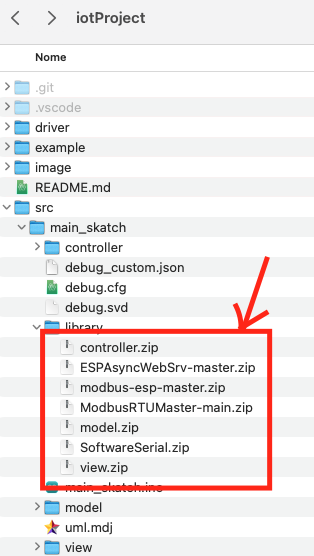
\includegraphics[width=0.3\linewidth]{../image/Library.png}
  \caption{Importazione delle librerie nell'Arduino IDE}
\end{figure}

\paragraph{} Altrimenti clonare la versione Portable del progetto disponibile al seguente link: \href{https://github.com/AlessioTommasi-supsi/iotProject/tree/portable}{iotProject-portable}.


\chapter{Diagramma UML}
\begin{figure}[H]
    \centering
    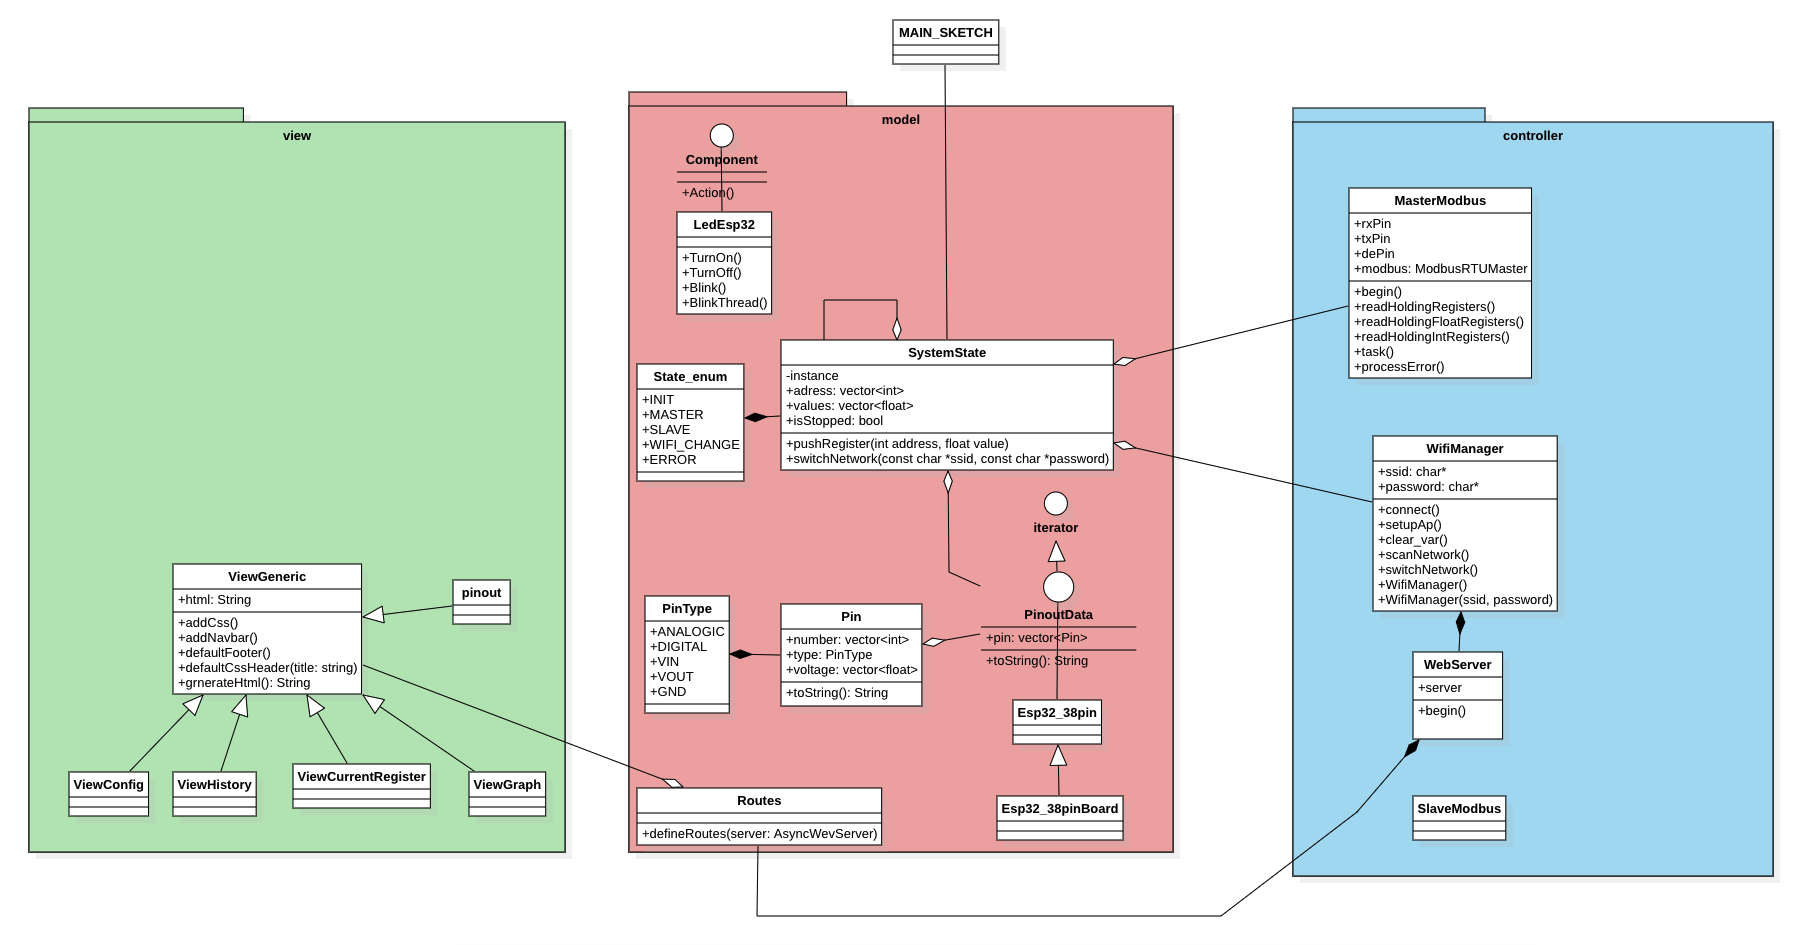
\includegraphics[width=\linewidth]{../image/uml.png}
    \caption{Diagramma UML del sistema}
\end{figure}

\chapter{Hardware}


\paragraph{Pin utilizzabili:}
asd
\section{Board Esam}
\subsection{Funzionamento}
\subsubsection{Multiplex}
\subsection{ hardware esterno posizionabile sulla board}
\subsubsection{MAX31865}
asd

\subsubsection{ESP32 38 Pin}

\begin{figure}[H]
    \centering
    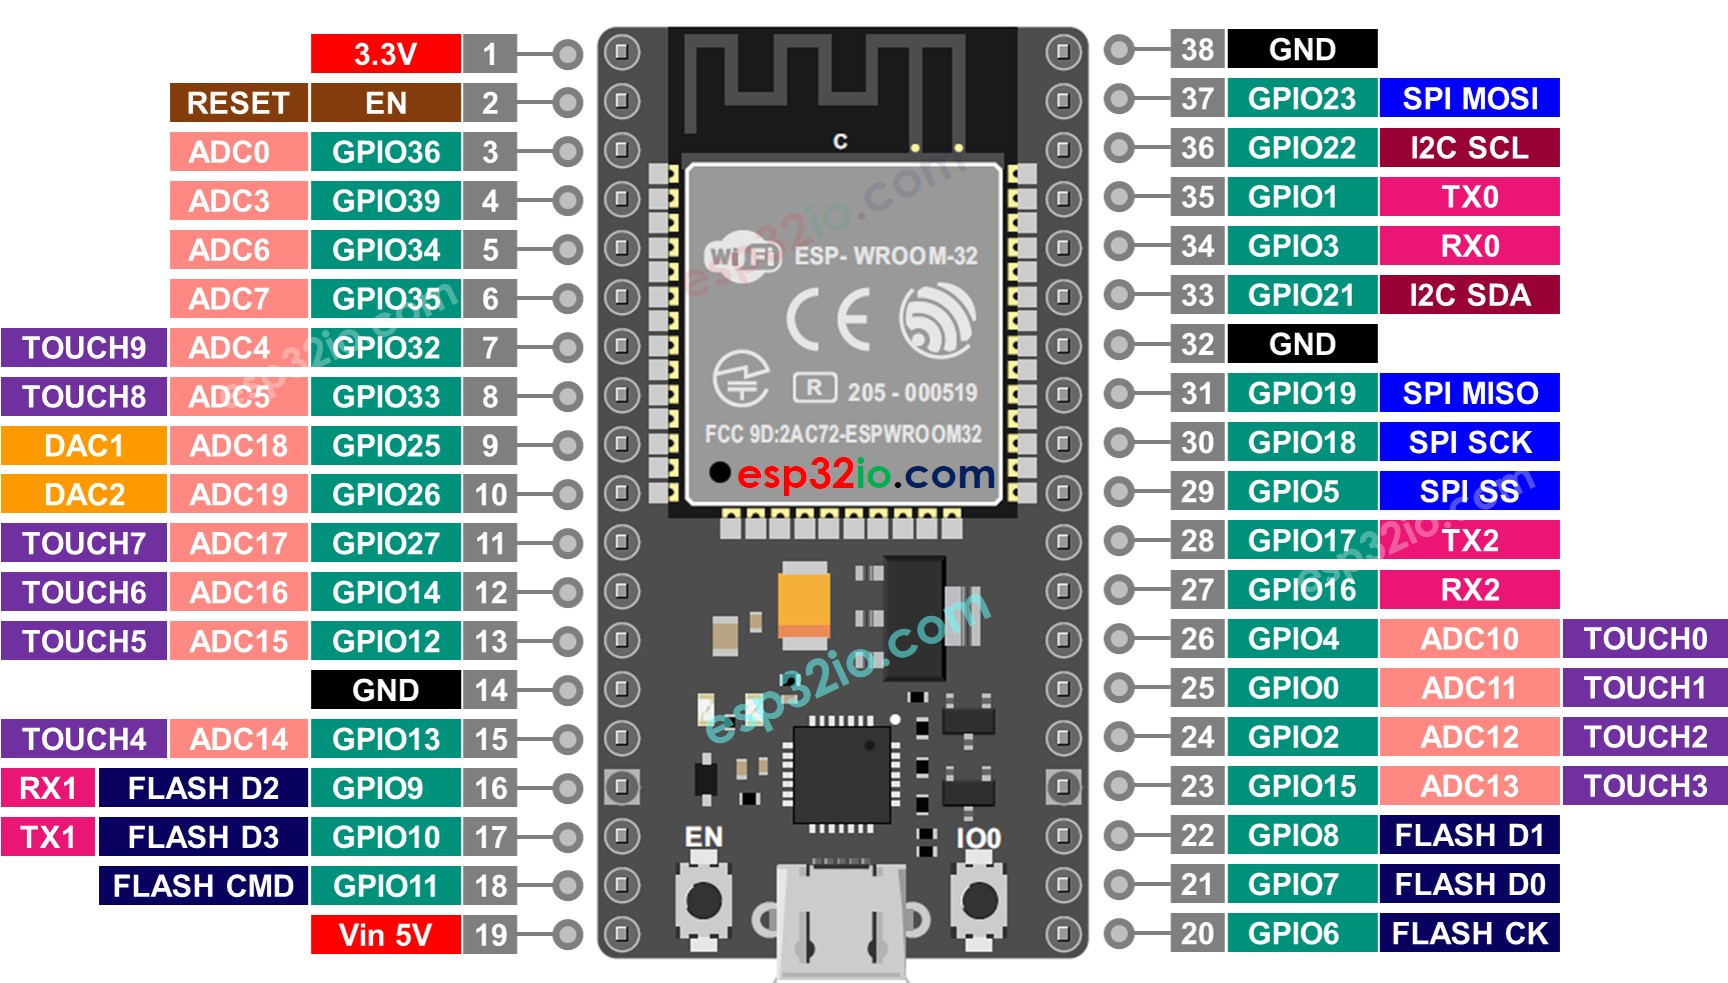
\includegraphics[width=\linewidth]{../image/ESP-38Pin-pinout.jpg}
    \caption{Pinout dell'ESP32-DOIT-DEV-KIT v1}
\end{figure}

\chapter{Modbus}

Il file utilizzato per testare lo slave è disponibile qui: \href{src/SLAVE\_EXAMPLE/modbusSlave2/modbusSlave2.ino}{modbusSlave2.ino}.

\begin{figure}[H]
    \centering
    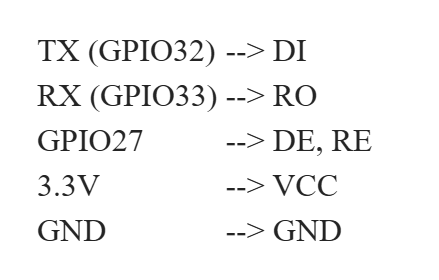
\includegraphics[width=\linewidth]{../image/SlavePinout.png}
    \caption{Pinout proposto per il dispositivo slave Modbus}
\end{figure}

\chapter{Attività}

\begin{longtable}{|p{0.35\textwidth}|p{0.65\textwidth}|}
\hline
\textbf{Attività} & \textbf{Descrizione} \\ \hline
\endfirsthead
\hline
\textbf{Attività} & \textbf{Descrizione} \\ \hline
\endhead
\hline
\endfoot
\textbf{Configurazione sensori di temperatura} & Configurare e integrare sensori di temperatura \textbf{PT100}, \textbf{PT1000} e \textbf{termocoppie} utilizzando moduli come \textbf{MAX31865} e \textbf{MAX31855}. \\ \hline
\textbf{Lettura segnali analogici} & Implementare la lettura di segnali analogici tramite gli ingressi \textbf{ADC} dell'ESP32 e eventuali moduli esterni. \\ \hline
\textbf{Gestione uscite digitali e analogiche} & Sviluppare la gestione delle uscite digitali e analogiche tramite l'ESP32. \\ \hline
\textbf{Comunicazione RS485 (Modbus RTU)} & Integrare la comunicazione \textbf{RS485} utilizzando il protocollo \textbf{Modbus RTU} per interfacciarsi con altri dispositivi. \\ \hline
\textbf{Server Web (Ethernet TCP/IP)} & Sviluppare un server \textbf{Web} basato su \textbf{Ethernet TCP/IP} per il monitoraggio e controllo remoto dei dati acquisiti. \\ \hline
\textbf{Datalogging} & Implementare un sistema di \textbf{datalogging} per salvare e storicizzare i dati raccolti dai sensori. \\ \hline
\textbf{Test e validazione} & Testare e validare il sistema attraverso simulazioni e test su hardware reale. \\ \hline
\end{longtable}



\end{document}
